\chapter{illustration}
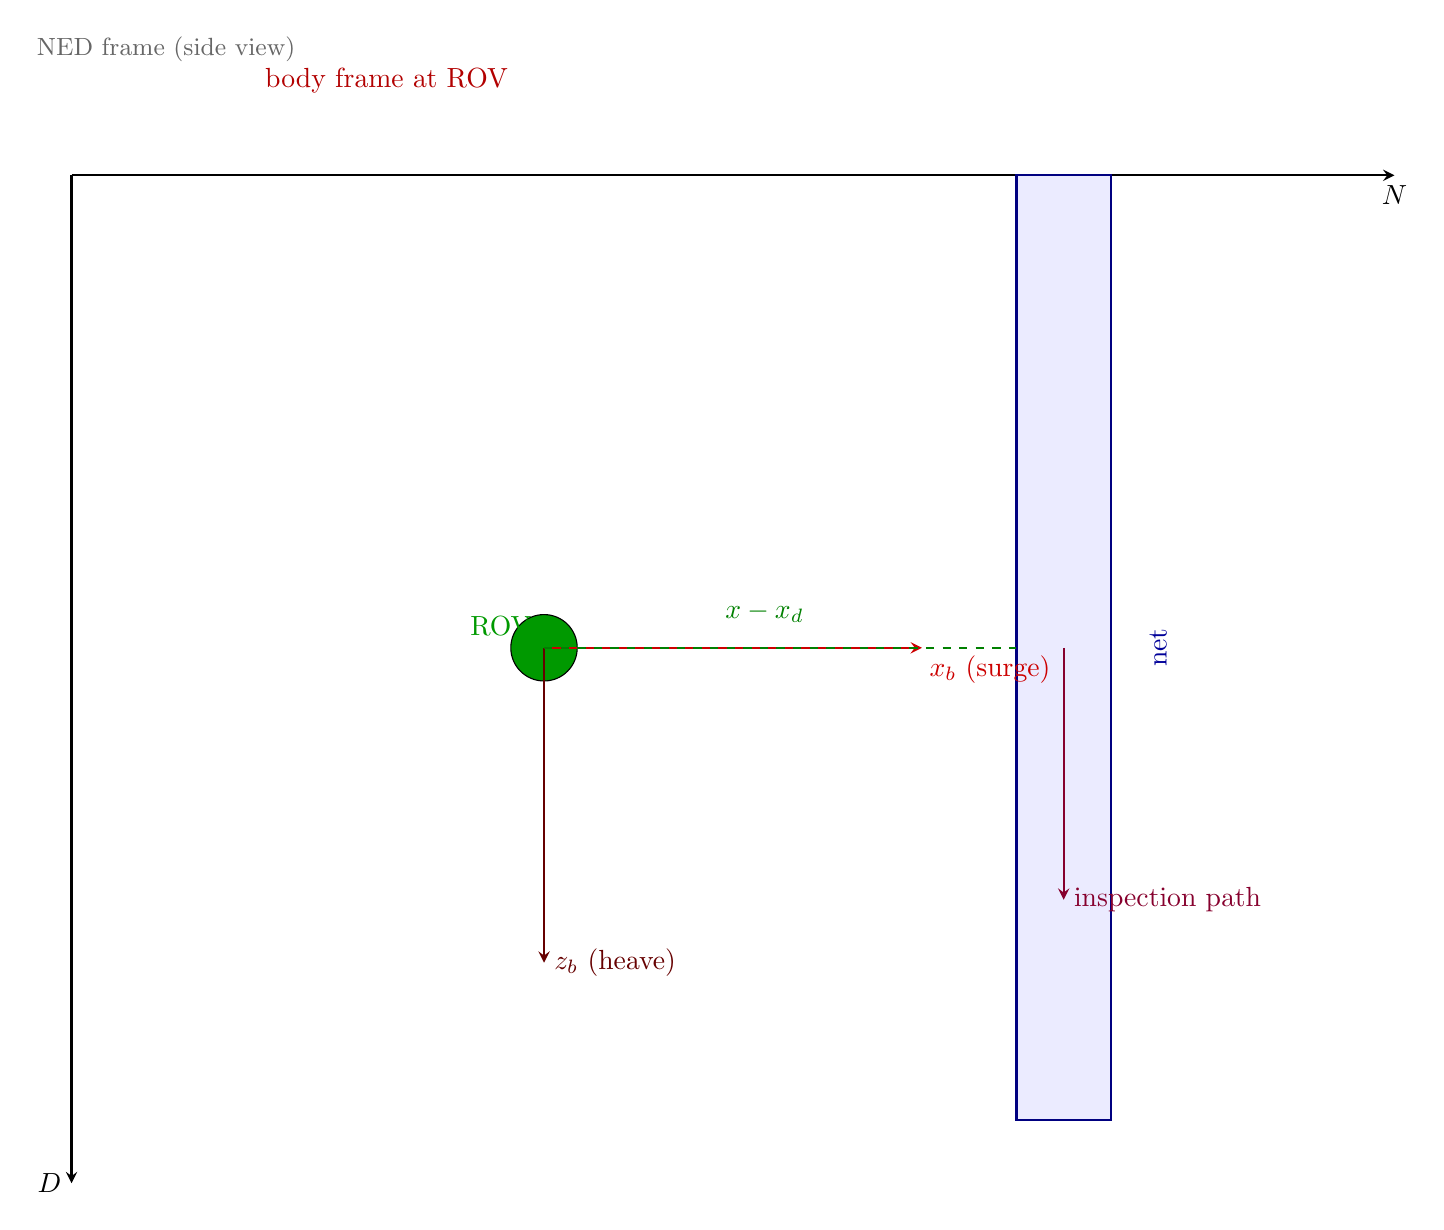
\begin{tikzpicture}[scale=4.0,>=stealth]

  %--- NED axes (N horizontal, D down) ---
  \draw[->,thick] (0,0) -- (4.2,0) node[below] {$N$};
  \draw[->,thick] (0,0) -- (0,-3.2) node[left] {$D$};
  \node[black!60] at (0.3,0.4) {\small NED frame (side view)};

  %--- Net plane ---
  \draw[fill=blue!8,draw=blue!50!black,thick]
        (3,0) -- (3,-3) -- (3.3,-3) -- (3.3,0) -- cycle;
  \node[blue!60!black,rotate=90] at (3.45,-1.5) {net};

  %--- ROV position ---
  \coordinate (rov) at (1.5,-1.5);
  \draw[fill=green!60!black] (rov) circle (3pt);
  \node[green!60!black,above left=1pt] at (rov) {ROV};

  %--- Body axes (x_b forward to net, z_b down) ---
  \draw[->,red!80!black,thick] (rov) -- ++(1.2,0)
      node[below right=-1pt] {$x_b$ (surge)};
  \draw[->,red!40!black,thick] (rov) -- ++(0,-1.0)
      node[right] {$z_b$ (heave)};

  %--- Distance to net (along body x) ---
  \draw[dashed,green!50!black,thick] (rov) -- (3,-1.5);
  \node[green!50!black,above] at (2.2,-1.45) {$x - x_d$};

  %--- Inspection motion along the net (up/down) ---
  \draw[->,purple!70!black,thick] (3.15,-1.5) -- ++(0,-0.8)
      node[right] {inspection path};

  %--- Annotate body frame ---
  \node[red!70!black] at (1.0,0.3) {body frame at ROV};

\end{tikzpicture}